\chapter{Nanotechnology and the Future of Computation, Storage and Perception}

\begin{center}
{\large\uppercase{Navakanta Bhat}}
%\footnote{Chief Mentor, email: rajendrabera@yahoo.com. Communicating author. The views expressed are those currently held by the author.}

\vskip -6pt

Professor and Chair, Centre for Nano Science and Engineering\\ Indian Institute of Science, Bangalore-560012
\end{center}

%\noindent\makebox[\textwidth]{
\includegraphics[width=1.05\paperwidth,height=17cm]{src/Figures/AI_powered_society.jpg}}

\newpage

\begin{multicols}{2}

\section{Historical Perspective and Current Status:}

The continued miniaturization of devices in the nanoscale regime, and the capability to manipulate the matter at these dimensions is expected to revolutionize the future systems for computation, storage and perception in the next few decades. Nanotechnology is not just a natural evolution of the miniaturization trend from sub-100 micrometer scale to sub-100 nanometer scale. The emergence of quantum effects at nanoscale, with a significant departure from  the continuum approximation of physical, chemical and biological processes, brings in exciting new possibilities with nanotechnology. In the next few decades, we will go beyond the conventional charge based, digital Silicon CMOS technology, and incorporate several emerging technologies that exploit nanoscale phenomena, to realize extremely powerful machines for high performance computation with augmented perception, mimicking the human brain and sensory organs. 

Fig.~\ref{chap1-fig1} depicts  the key milestones in the evolution of compute engines. The bulky and power hungry vacuum tubes used in one of the early digital computers, ENIAC, resulted in rudimentary computation capabilities with the computer weighing 30 tons and consuming 200 kW power. This was certainly not a scalable technology. The invention of semiconductor transistor in 1947 was an inflexion point in the history of miniaturization. This was followed by the invention of the first integrated circuit (IC), a decade later in 1958. However, most of the early ICs were only memory chips and the community was concerned as to what one would do with all those storage devices. Then, the first microprocessor IC invented in 1971,  changed the landscape completely. The Intel 4004, a 4 bit microprocessor was realized on 10 $\mu,\mbox{m}$ PMOS technology, with a chip size of 12 mm2 and power consumption of 1W. This was soon followed by migration to  NMOS technology (Intel 8080 in 1974) and CMOS technology (Intel 80386 in 1985).  As exemplified by the famous Moore’s law, the miniaturization trend has continued with CMOS technology scaling, resulting in a new generation of manufacturing technology introduced every 2 to 3 years. This technology scaling,  coupled with several innovations in system and circuit architectures, has fuelled the growth of more and more powerful compute engines over the years. For instance, in 2013, the CMOS technology went through another big change with the introduction of 3 dimensional (3D) FinFETs, departing from the conventional planar MOSFETs (Fig.~\ref{chap1-fig2}). By this time, the CMOS technology was also enabled by innovations in nanomaterials technology such as strained Silicon-Germanium channel, $\mbox{HfO}_2$ high-k gate dielectric with atomically engineered interface. On the architectural front, the introduction of multi-core processors, brought in an unprecedented computing capabilities, even to the hand held devices.  

\begin{figure}[H]
\centering
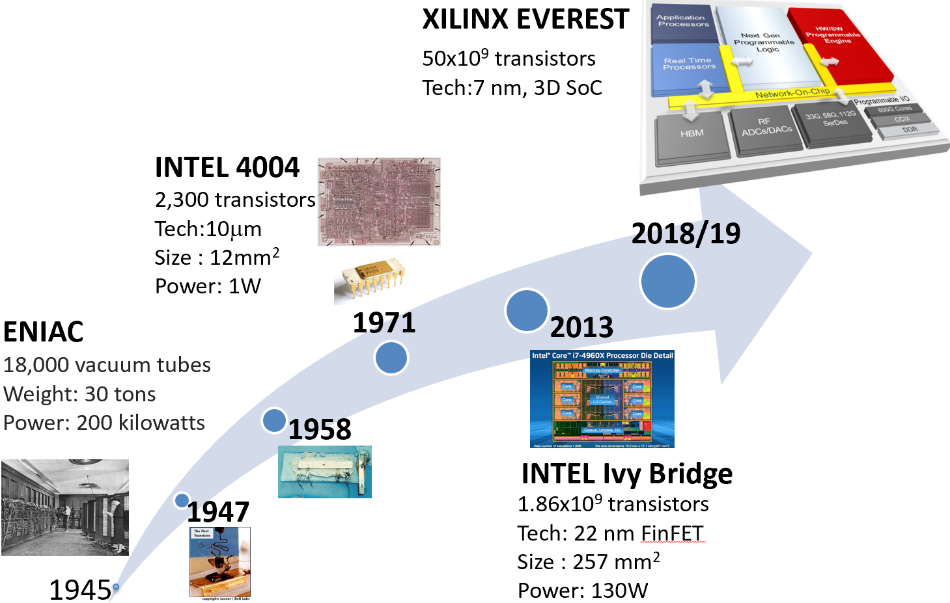
\includegraphics{src/Figures/chap1/chap1-fig01.jpg}
\caption{Evolution of computation chips [the illustrative images are from Intel and Xilinx]}\label{chap1-fig1}
\end{figure}

\begin{figure}[H]
\centering
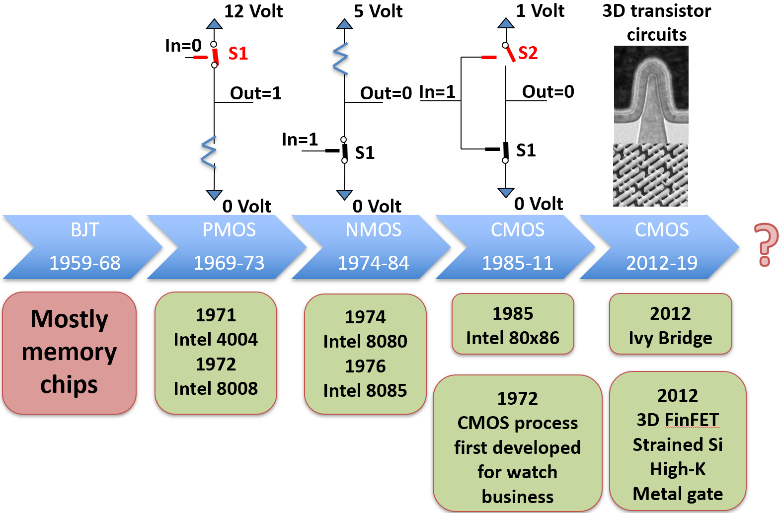
\includegraphics{src/Figures/chap1/chap1-fig02.jpg}
\caption{Evolution of transistor technology with an illustration of inverter implementation}\label{chap1-fig2}
\end{figure}

The Everest chip from  XILINX, on 7nm CMOS technology with 3D System on Chip fabric, packs 50 billion transistors on single chip, illustrating an amazing technological achievement. It should be recognized that in conjunction to miniaturization, the integration of  exponentially large number of transistors is primarily responsible for today’s high performance compute and storage chips. As shown in Fig.~\ref{chap1-fig3}, over the last 5 decades, while the “feature size” of transistors has scaled down by  3 orders of magnitude $(10^{-3})$, the number of components on chip has been increased by 7 orders of magnitude $(10^7)$. In conjunction with migration from microtechnology to nanotechnology, we have also moved from small scale integration (SSI) to Very Large Scale Integration (VLSI) or Giga Scale Integration (GSI).

\begin{figure}[H]
\centering
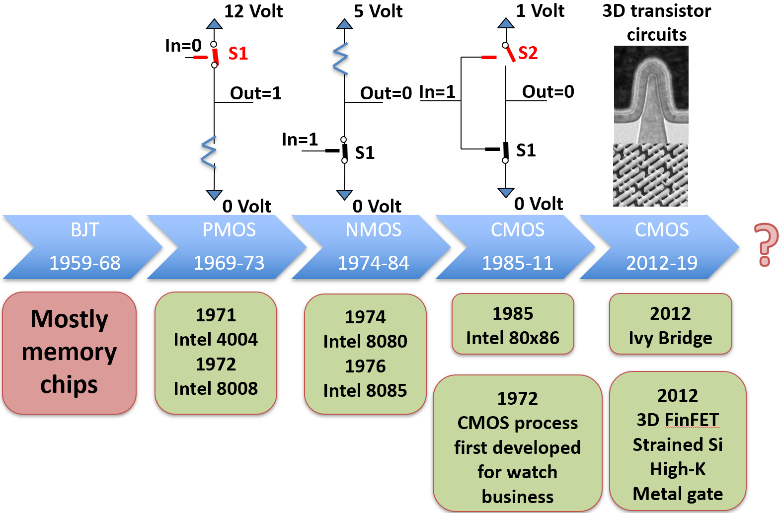
\includegraphics{src/Figures/chap1/chap1-fig02.jpg}
\caption{Transistor size scaling, coupled with exponential increase of transistor count}\label{chap1-fig3}
\end{figure}

In addition to the underlying nanoscale CMOS technology and ever evolving system and circuit architecture, the highly complex and powerful chips of today owe it to another key enabler, namely the Electronics Design Automation (EDA) using Computer Aided Design (CAD) tools. It is not hard to appreciate that the designing of giga scale integrated circuits would be impossible without sophisticated CAD tools. In late 70s, the handcrafting of the transistors on a chip, turned out to be unmanageable. This led to the emergence of hierarchical abstraction of various components of the chip at behavioural, structural, functional and physical level. The design concepts put forth by Mead and Convey, eventually led to commercial CAD tools to assist in the design of complex chips. Today there is an interesting symbiosis: the advanced CAD tools enabling advanced chips, which in turn enable advanced compute engines that are capable of supporting further advances in CAD tools. The CAD tools have matured so much that the design of a complex chip is akin to writing a software code, through hardware description languages such as Verilog and VHDL. Through the accurate modelling abstraction at different levels, it is possible to achieve first pass success, from specification to the fabrication of a chip, through logic synthesis and layout synthesis tools (Fig.~\ref{chap1-fig4}). For any other emerging nanotechnology option to be  successful, it is extremely important to have similar CAD tools to manage complex designs. 

\begin{figure*}[!t]
\centering
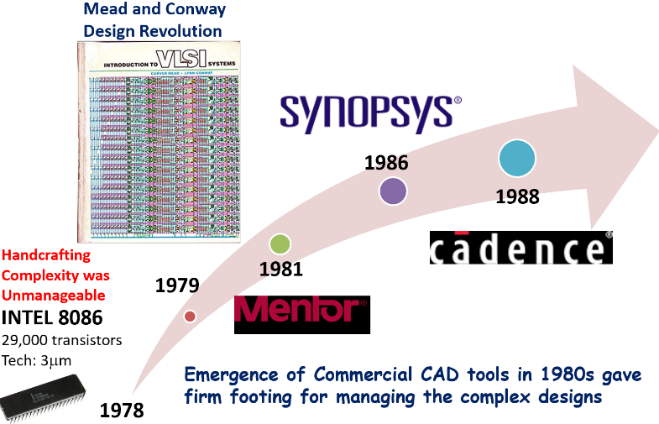
\includegraphics{src/Figures/chap1/chap1-fig04a.jpg}\qquad\qquad
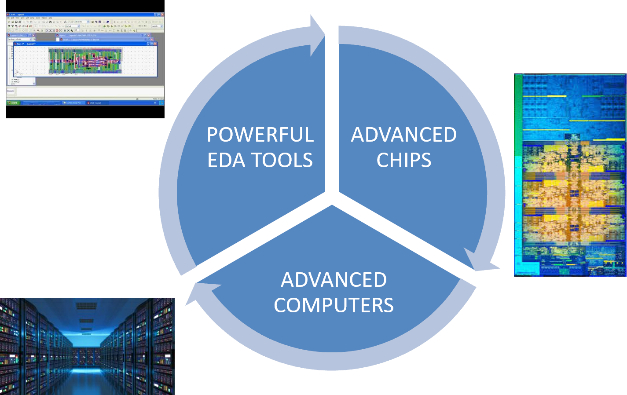
\includegraphics{src/Figures/chap1/chap1-fig04b.jpg}\\[15pt]
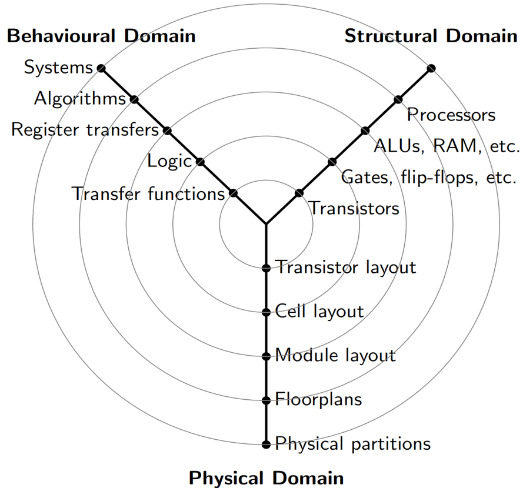
\includegraphics{src/Figures/chap1/chap1-fig04c.jpg}\qquad\qquad
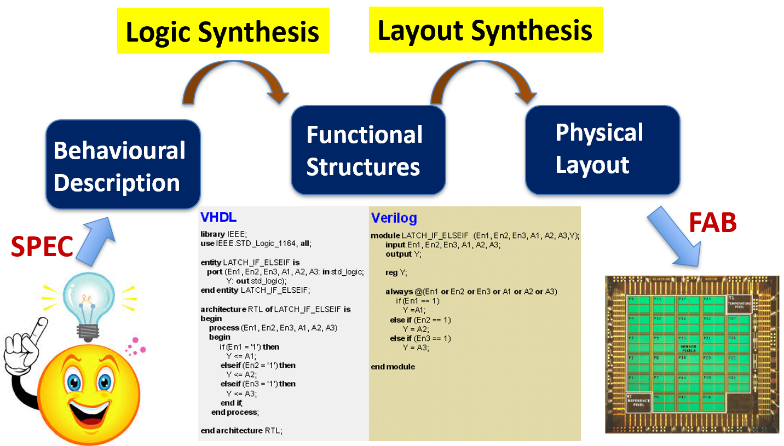
\includegraphics{src/Figures/chap1/chap1-fig04d.jpg}
\caption{The emergence of CAD tools for the design of complex chips, with a symbiotic positive feedback between EDA tools, advanced chips and high performance computers.  “Gajski-Kuhn Y chart” illustrating abstraction at behavioural, structural and physical domains. EDA tools enabling the “chip design compilers”}\label{chap1-fig4}
\end{figure*}

\section{Future Directions:} 

\end{multicols}
